\section{Mockups}
Um allen Projektbeteiligten ein Bild der zukünftigen Applikation zu vermitteln, sind für die wichtigsten Seiten Mockups entstanden. In diesem Abschnitt wird auf zwei Ansichten in der Connection Verwaltung eingegangen. Alle anderen Mockups sind im Anhang auf der Seite \pageref{Mockups} ersichtlich.

\subsection{Connection Übersicht}
\begin{figure}[H]
	\centering
	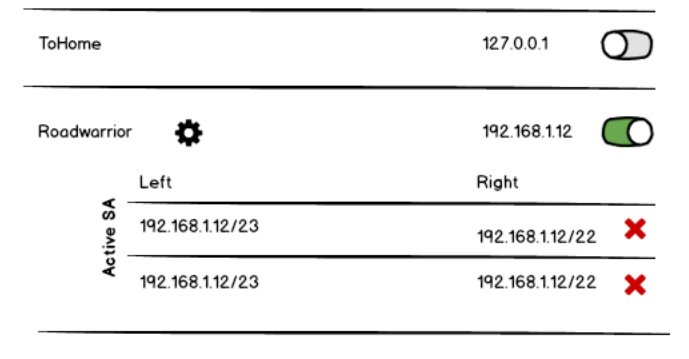
\includegraphics[width=330pt]{images/mockups/short_con_overview.jpg}
	\caption{Ausschnitt aus der Connection Übersicht}
\end{figure}

Die erstellten Verbindungen werden in Zeilenform untereinander angeordnet. Es gibt einen zentralen Toggle Button, der die Verbindung aktiviert/deaktiviert und gleichzeitig den Verbindungsstatus anzeigt. Sobald die Verbindung gestartet wurde, wird die Verbindungszeile erweitert und die aktiven SA's angezeigt.

\subsection{Connection hinzufügen}
\noindent\begin{minipage}{0.55\textwidth}
    \begin{figure}[H]
    	\centering
    	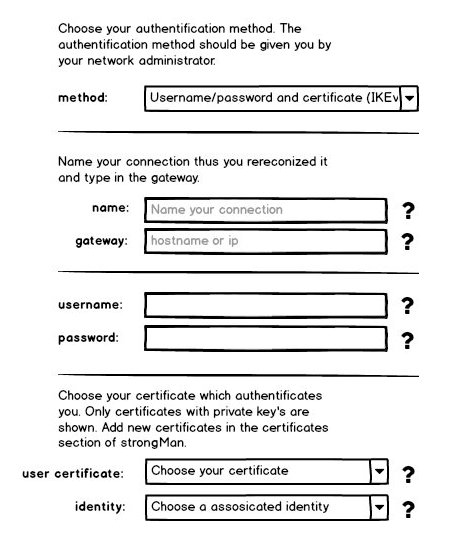
\includegraphics[width=240pt]{images/mockups/short_con_config.jpg}
    	\caption{Ausschnitt aus dem Connection hinzufügen}
    \end{figure}
\end{minipage}
\hfill
\begin{minipage}{0.45\textwidth}
Nachdem der Benutzer die Authentifizierungsmethod ausgewählt hat (hier nicht ersichtlich), erscheinen unterhalb die entsprechenden Eingabefelder.

Das Konfigurieren einer Verbindung wurde so einfach wie möglich gestaltet. Der Benutzer soll kurz vor jeder Eingabe informiert werden, welche Nutzen das entsprechende Feld hat und sich bei Schwierigkeiten an Hilfetexten informieren können (Klick auf die Fragezeichen).
\end{minipage}


\section{Usability Tests}